
% This LaTeX was auto-generated from MATLAB code.
% To make changes, update the MATLAB code and republish this document.

\documentclass{article}
\usepackage{graphicx}
\usepackage{color}

\sloppy
\definecolor{lightgray}{gray}{0.5}
\setlength{\parindent}{0pt}

\begin{document}

    
    
\subsection*{Contents}

\begin{itemize}
\setlength{\itemsep}{-1ex}
   \item ELEC 4700 Assignment 2: Finite Difference Method
   \item Part 1
   \item Part 2
\end{itemize}


\subsection*{ELEC 4700 Assignment 2: Finite Difference Method}

\begin{par}
Dilsha Appu-Hennadi, 101107857 Feb. 18, 2022 Latest rev. Feb. 23, 2022
\end{par} \vspace{1em}
\begin{verbatim}
clear all
clearvars
clearvars -GLOBAL
close all
format shorte
\end{verbatim}
\begin{par}
In this assignment we will be solving Laplacce's Equation for electrostatic potential within an L-by-W rectangular region.
\end{par} \vspace{1em}
\begin{verbatim}
global regL regW L W

regL = 200e-9;
regW = 100e-9;

L = 60;
W = 40;

nx = L;
ny = W;
\end{verbatim}


\subsection*{Part 1}

\begin{par}
For Part 1, we will use the matrix form of the Finite Difference Method to solve for the electrostatic potential in the rectangular region. For this part, we will use: $$ \nabla^2 V = 0 $$. For a) $$ V = V_0 $$ at $$ x = 0 $$ and $$ V = 0 $$ at $$ x = L $$ we will also assume the top and bottom boundaries are insulated - i.e. $$ \frac{dV}{dy} = 0 $$.
\end{par} \vspace{1em}
\begin{par}
$$ \nabla^2 V  = 0 $$
\end{par} \vspace{1em}
\begin{par}
$$ \frac{d^2 V}{dx^2} + \frac{d^2 V}{dy^2} = 0 $$
let
$$ \delta x = \delta y = \delta = 1 $$
$$ V_{m+1,n} + V_{m-1,n} + V_{m,n+1} + V_{m,n-1} - 4V_{m,n} = 0 $$
\end{par} \vspace{1em}
\begin{verbatim}
assign2part1a;
\end{verbatim}

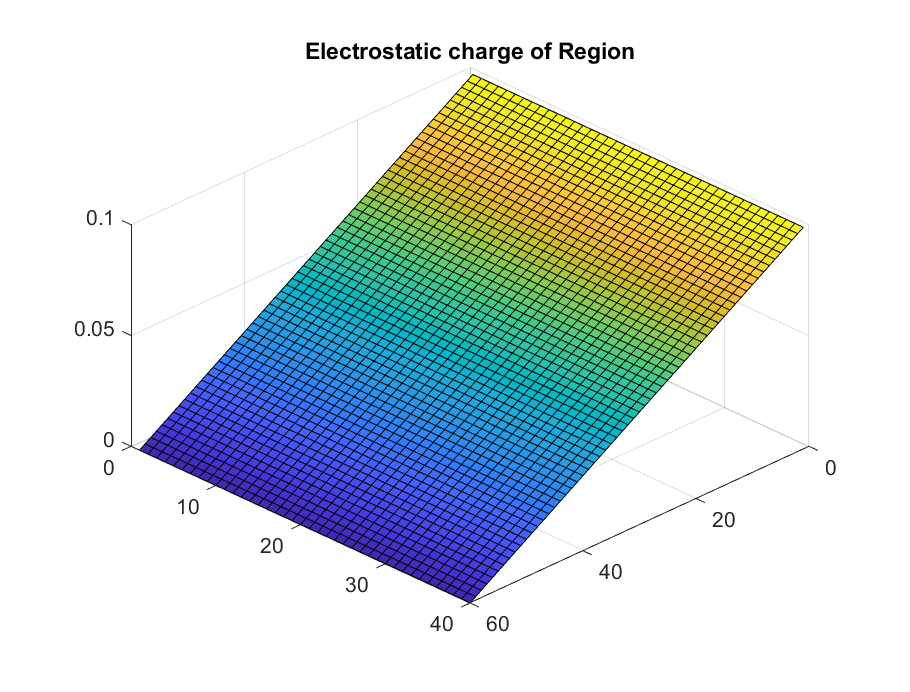
\includegraphics [width=4in]{main_01.eps}
\begin{par}
As expected, the electrostatic charge of the region varies linearly from V\_0 (which was set to 1V) down to 0 volts.
\end{par} \vspace{1em}
\begin{par}
For b), BCs will be set to:
\end{par} \vspace{1em}
\begin{par}
$$ V = V_0 $$ at $$ x = 0,L $$ and $$ V = 0 $$ at $$ y = 0,W $$
\end{par} \vspace{1em}
\begin{verbatim}
% assign2part1b;
\end{verbatim}
\begin{par}
Now we see that the left and right sides of the region are set to V\_0 (which is again 1V) and the top and bottom sides of the region are 0V. Because of this, there is a very quick drop in the charge moving away from either the left or right side, especially in the corners.
\end{par} \vspace{1em}
\begin{par}
For this case we tried solving the electrostatic problem using the Finite Difference Method from part A as well as numerically calculating the solution using an infinite series (although the summation wasn't actually infinite, but rather a large number of summations were done). As we can see, the two subplots look very similar to each other. However, upon closer inspection, the numerical solution is not quite as smooth along the top edge. This is due to the fact that we were unable to take an infinite number of summations as we see that few summations provide a worse plot, while more summations provide a more accurate solution.
\end{par} \vspace{1em}


\subsection*{Part 2}

\begin{par}
In this part, we will investigate the Finite Difference Method to solve for the current flow through the rectangular region from Part 1 using: $$ \nabla \left( \sigma_{x,y} \nabla V \right) = 0 $$ As with Part 1, we will assume boundary conditions of the area will be the same as case 1: $$ V = V_0 $$ at $$ x = 0 $$ and $$ V = 0 $$ at $$ x = L $$
\end{par} \vspace{1em}
\begin{verbatim}
% assign2part2
\end{verbatim}
\begin{par}
For this part, we had gone back to the same boundary conditions as case a) in Part 1, only this time there are sections of the region with a different conductivity. In the real world, this may simulate impurities within our Si crystal structure. We have a conduction map laid out to provide a visual on what the conduction of the region looks like. For the most part, it's constant, however we've now added two boxes with a much lower conductivity compared to the surrounding area.
\end{par} \vspace{1em}
\begin{par}
Next to the conduction map, we have a plot of the electrostatic charge which for the most part looks like the plot obtained for case a) in Part 1. However, we now see a much sharper slope where the two boxes are. This would make sense are the electrostatic charge would depend on the conductivity and thus we should expect to see a difference at the location of the two boxes.
\end{par} \vspace{1em}
\begin{par}
The two bottom subplots are graphs of the electric field present in the material and the current density. We see from the Electric field plot that there is a significant E-field where the two boxes are. This makes sense as there is a significant difference in electric charge one either side of the boxes and low conductivity of the boxes make it act similar to dielectric material. Conversly, there is a high current density between the two boxes (within the bottle-neck) as a lot of electrons are being funneled through the path as they move around  the region.
\end{par} \vspace{1em}
\begin{par}
We can observe how the current through the region is effected by the mesh size, the different types of bottle necks and varying conductivity.
\end{par} \vspace{1em}
\begin{verbatim}
currVsMesh = [0.0057 30*20; 0.0027 60*40; 0.0019 90*60; 0.0014 120*80; 0.0011 150*100];
currVsBotNeck = [0.0032 0.8*W; 0.0030 0.6*W; 0.0027 0.4*W; 0.0024 0.2*W; 0.0021 0.1*W];
currVsCond = [6.3988e-4 0.2; 9.2337e-4 0.3; 0.0012 0.4; 0.0015 0.5; 0.0017 0.6; 0.0020 0.7; 0.0022 0.8; 0.0025 0.9; 0.0027 1];
\end{verbatim}
\begin{par}
The plot below shows how the current measurement changes as the mesh size is adjusted. We see that the current starts high and gets lower as it levels out at a smaller current.
\end{par} \vspace{1em}
\begin{verbatim}
figure(4)
plot(currVsMesh(:,2),currVsMesh(:,1))
title('Current vs Mesh size')
xlabel('Mesh size')
ylabel('Current')
\end{verbatim}

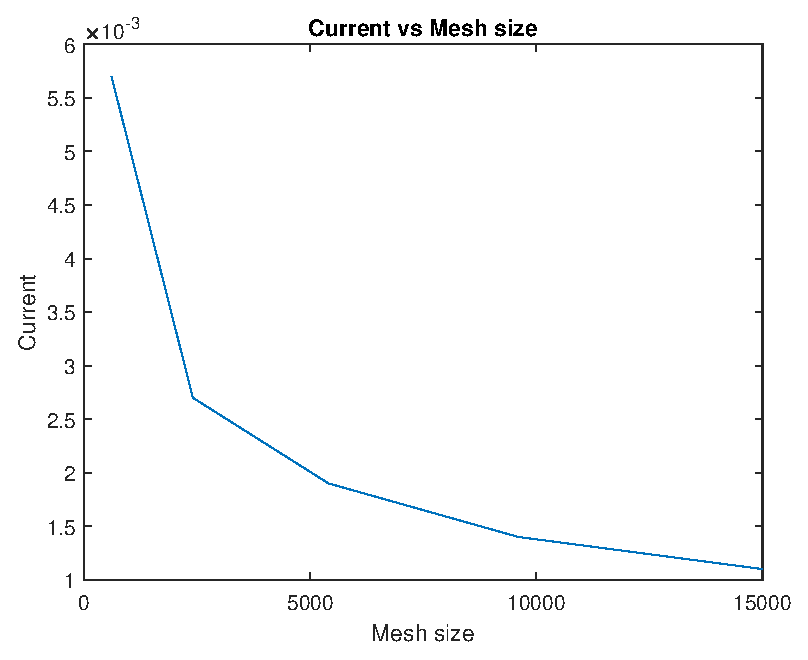
\includegraphics [width=4in]{main_02.eps}
\begin{par}
The next graph depicts how current changes with different bottle neck sizes. As the current calculation involves taking the average of the current density and multiplying by the area of the region, the higher density at lower bottle-neck widths creates what appreas to be a higher current.
\end{par} \vspace{1em}
\begin{verbatim}
figure(5)
plot(currVsBotNeck(:,2),currVsBotNeck(:,1))
title('Current vs Bottle Neck Size')
xlabel('Size of Bottle Neck')
ylabel('Current')
\end{verbatim}

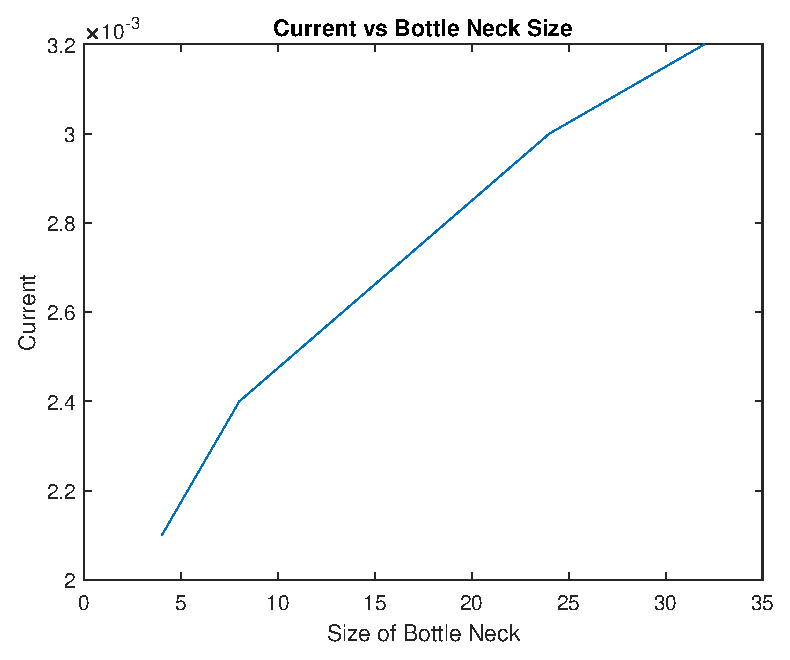
\includegraphics [width=4in]{main_03.eps}
\begin{par}
In the final plot, we have a graph of the current and conductivity. We see that the current in the system varies linearly with the conductivity and as conductivity increases, the current will increase. This makes intuitive sense as higher conductivities will allow for easier flow of charge carriers.
\end{par} \vspace{1em}
\begin{verbatim}
figure(6)
plot(currVsCond(:,2),currVsCond(:,1))
title('Current vs Conduction')
xlabel('Conduction of High Conduction Area')
ylabel('Current')
\end{verbatim}

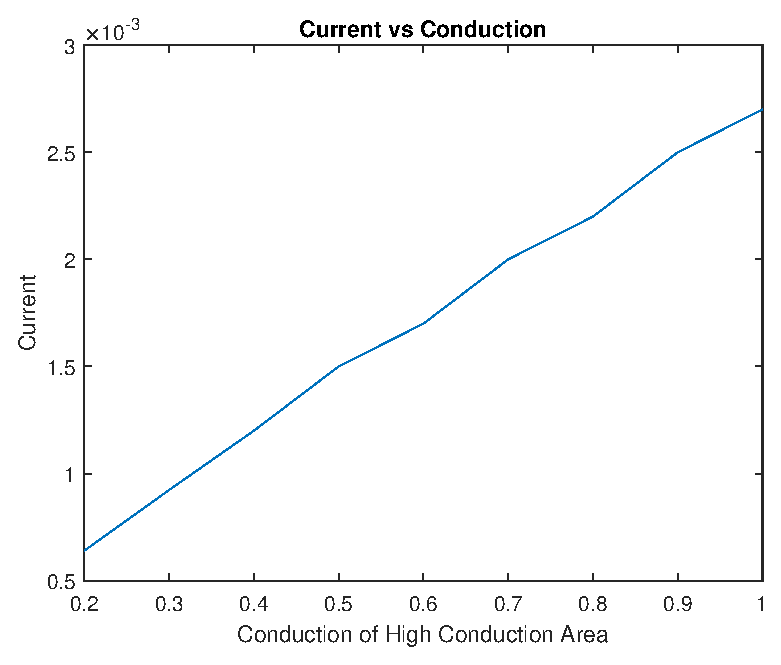
\includegraphics [width=4in]{main_04.eps}



\end{document}

